% !TEX root = ./rosbook_jp.tex
%-------------------------------------------------------------------------------
\chapterimage{chapter_head_4.pdf}

%-------------------------------------------------------------------------------
\chapter{ROS コマンド}\index{ROS コマンド}

ROSは、Ubuntuのコマンドラインインタフェース (CLI)であるシェル(shell)環境で、様々なコマンドを使用して、ファイルシステムの利用、ソースコードの編集、ビルド、デバッグ、パッケージ管理などを行う。ROSを利用するには、基本的なLinuxコマンドに加えて、ROS固有のコマンド注1を修得する必要がある。本章では、それらのROS固有のコマンドを、ROSシェルコマンド、ROS実行コマンド、ROS情報コマンド、ROS catkinコマンド、ROSパッケージのコマンドに分けて説明する。主な用途を以下に示す。

\begin{itemize}
\item ROSシェルコマンド: コピーなどのファイル操作やディレクトリ操作
\item ROS実行コマンド: ノードの実行
\item ROS情報コマンド: ノードやメッセージ情報の表示
\item ROS catkinコマンド: パッケージのビルド
\item ROSパッケージのコマンド: パッケージのインストールや依存関係の表示
\end{itemize}

なお、コマンドの後のアスタリスクは、そのコマンドの使用頻度を表している。

%-------------------------------------------------------------------------------
\section{ROSシェルコマンド}\index{ROSシェルコマンド}

ROSシェルコマンドはrosbashと呼ばれ、Linuxで一般的に使用されるbashシェルコマンドに類似した、ROS特有のシェルコマンドである。

\vspace{\baselineskip}
\noindent
\begin{description}
\item[roscd](★★★)ros+cd(changes directory):指定されたROSパッケージのディレクトリに移動
\item[rosls] (★☆☆)ros+ls(lists files):ROSパッケージのファイルリストを確認
\item[rosed](★☆☆)ros+ed(editor):ROSパッケージのファイルを編集
\item[roscp] (★☆☆)ros+cp(copies files):ROSパッケージのファイルをコピー
\item[rospd](☆☆☆)ros+pushd:ROSディレクトリインデックスにディレクトリを追加
\item[rosd](☆☆☆)ros+directory:ROSディレクトリインデックスを確認
\end{description}

このうち、頻繁に使用されるroscd、rosls、rosedコマンドについて詳しく述べる。

\begin{exercise}[ROSシェルコマンドを使用できる環境]
    ROSシェルコマンドは、次のコマンドでrosbashがインストールされており、「source /opt/ros/<ros distribution>/setup.bash」が設定された端末で使用できる。2章のROSのインストールが正しく行われていれば、すぐに使用できる。
  \begin{lstlisting}[language=ROS]
  $ sudo apt-get install ros-<ros distribution>-rosbash
  \end{lstlisting}
  例えば、ROSのバージョンがindigoであれば以下のコマンドである。
  \begin{lstlisting}[language=ROS]
  $ sudo apt-get install ros-indigo-rosbash
  $ source /opt/ros/indigo/setup.bash
  \end{lstlisting}
\end{exercise}

%-------------------------------------------------------------------------------
\subsection{roscd:ROSパッケージのディレクトリへ移動}

roscdは、パッケージの保存先のディレクトリに移動するコマンドである。自分が作成したパッケージやインストールしたパッケージの名前を、パラメータとしてこのコマンドに続けて入力すると、そのパッケージの置かれたディレクトリに移動する。使用頻度は非常に高い。

\begin{itemize}
\item roscd [パッケージ名]
\end{itemize}

下の例は、ROSのインストールフォルダにあるturtlesimパッケージに移動している様子である。

\begin{lstlisting}[language=ROS]
$ roscd turtlesim
/opt/ros/indigo/share/turtlesim$
\end{lstlisting}

なお、上の例では、関連するパッケージであるros-indigo-turtlesimがインストールされている必要がある。インストールされていない場合は、次のコマンドでインストールできる。

\begin{lstlisting}[language=ROS]
$ sudo apt-get install ros-indigo-turtlesim
\end{lstlisting}

%-------------------------------------------------------------------------------
\subsection{rosls:ROSファイルのリスト表示}

roslsは指定されたROSパッケージ内のファイルの一覧を表示するコマンドである。パッケージ名をこのコマンドに続けて入力すると、そのパッケージを検索し、パッケージ内のファイルの一覧を表示する。

\begin{itemize}
\item  rosls [パッケージ名]
\end{itemize}

\begin{lstlisting}[language=ROS]
$ rosls turtlesim
cmake images msg package.xml srv
\end{lstlisting}

%-------------------------------------------------------------------------------
\subsection{rosed:ROSファイルの編集}

rosedはパッケージ内のファイルを編集するときに使用するコマンドであり、ユーザーが設定したエディタでファイルを開く。比較的簡単な内容を手軽に修正するときに使用する。この時、使用されるエディタは、「~/.bashrc」ファイルに「export EDITOR= 'nano'」のように指定する。

\begin{itemize}
\item   rosed [パッケージ名] [ファイル名]
\end{itemize}

\begin{lstlisting}[language=ROS]
$ rosed turtlesim package.xml
\end{lstlisting}

%-------------------------------------------------------------------------------
\section{ROS実行コマンド}\index{ROS実行コマンド}

ROS実行コマンドは、ROSノードの実行を制御する。特にroscoreはROSネームサーバであるROSマスター、標準出力・標準エラー出力のためのrosout、パラメータを管理するパラメータサーバを同時に起動するものであり、他のノードの実行前に実行する必要がある。ノードの実行コマンドには、rosrunとroslaunchがある。rosrunは単一のノードを実行するものであり、roslaunchは複数のノードを実行する。また、roscleanは、ノードの実行時に記録されるログを削除するコマンドである。

\vspace{\baselineskip}
\noindent
\begin{description}
\item[roscore](★★★)ros+core:ROSマスター(ROSネームサーバ)、rosout(標準出力stdout/標準エラー出力stderr)、パラメータサーバ(パラメータ管理)の起動
\item[rosrun](★★★)ros+run:パッケージの一つのノードを実行
\item[roslaunch](★★★)ros+launch:パッケージの複数のノードを同時実行
\item[rosclean](★★☆)ros+clean:rosログファイルを確認、削除
\end{description}

%-------------------------------------------------------------------------------
\subsection{roscore:ROSマスター、rosout、パラメータサーバの起動}

roscoreは、ノード間のメッセージ通信の接続情報を管理するROSマスターを起動するコマンドである。起動されたROSマスターはXMLRPCのサーバとなる。ROSマスターは、ROSの使用にあたって最初に起動しておく必要がある。roscoreを実行すると、ユーザーが設定した「~/.bashrc」中のROS\_MASTER\_URIをマスターURIとし、ROSマスターが立ち上がる。

\setcounter{num}{0}

\begin{lstlisting}[language=ROS]
$ roscore
... logging to /home/xxx/.ros/log/f4b17da6-ecda-11e4-a7bf-d43d7e970cb0/roslaunch-rt-18869.log \stepcounter{num}\circled{\thenum} )
Checking log directory for disk usage. This may take a while.
Press Ctrl-C to interrupt  \stepcounter{num}\circled{\thenum}
Done checking log file disk usage. Usage is <1GB.

started roslaunch server http://192.168.4.100:47915/
ros_comm version 1.11.10


SUMMARY
========

PARAMETERS
 * /rosdistro: indigo \stepcounter{num}\circled{\thenum}
 * /rosversion: 1.11.10 \stepcounter{num}\circled{\thenum}

NODES

auto-starting new master
process[master]: started with pid [18881]
ROS_MASTER_URI=http://192.168.4.100:11311/ \stepcounter{num}\circled{\thenum}

setting /run_id to f4b17da6-ecda-11e4-a7bf-d43d7e970cb0
process[rosout-1]: started with pid [18894]
started core service [/rosout] \stepcounter{num}\circled{\thenum}
\end{lstlisting}

上記の出力結果の太字部分から、①「/home/xxx/.ros/log/」フォルダにログが保存されていること、②<Ctrl>+<C>でroscoreを終了ができること、③「/rosdistro」と④「/rosversion」がパラメータとしてパラメータサーバに登録されたこと、⑤ROS\_MASTER\_URIの情報、⑥「/rosout」ノードが実行されたことなどが確認できる。

\begin{exercise}[ログの保存場所]
上の例ではlogが保存される場所が「/home/xxx/.ros/log/」(xxxはユーザー名)となっているが、ROS\_HOME環境変数を設定することで任意の場所に保存できる。変数が設定されていない場合は「/home/xxx/.ros/log/」に記録される。
\end{exercise}

%-------------------------------------------------------------------------------
\subsection{rosrun:ROSノードの実行}

rosrunは、指定したパッケージ内の1つのノードを実行するコマンドである。

\begin{itemize}
\item   rosrun [パッケージ名] [ノード名]
\end{itemize}

以下の例では、turtlesimパッケージ内のturtlesim\_nodeノードを実行する。実行結果を図4-1に示す。

\begin{lstlisting}[language=ROS]
$ rosrun turtlesim turtlesim_node
[INFO] [1430205691.820701916]: Starting turtlesim with node name /turtlesim
[INFO] [1430205691.827666004]: Spawning turtle [turtle1] at x=[5.544445], y=[5.544445], theta=[0.000000]
\end{lstlisting}

\begin{figure}[h]
  \centering
  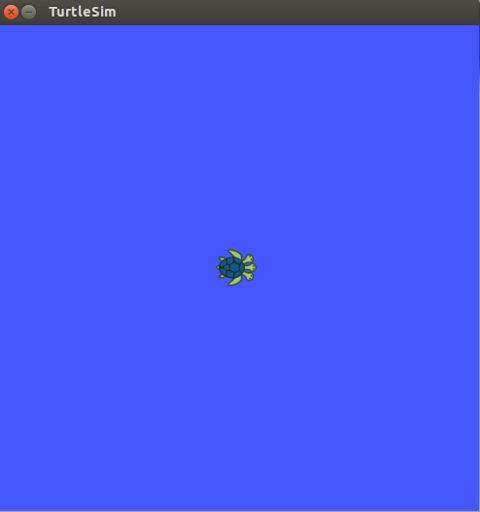
\includegraphics[width=\columnwidth]{pictures/chapter4/pic_04_01.png}
  \caption{turtlesim\_nodeノードを実行した様子}
\end{figure}


%-------------------------------------------------------------------------------
\subsection{roslaunch:複数のROSノードの実行}

roslaunchは、指定されたパッケージから1つ以上のノードを実行するコマンドである。

\begin{itemize}
\item   roslaunch [パッケージ名] [launchファイル名]
\end{itemize}

roslaunchは、複数のノードを実行する際に非常に有用であり、頻繁に使用されるノードの実行方法である。launchファイルの作成法については、6.5節「roslaunchの使い方」で詳細に取り上げる。
下の例のようにopenni\_launchパッケージ内のopenni.launchファイルを実行するだけで、camera\_nodelet\_manager、depth\_metric、depth\_metric\_rect、depth\_pointsなどの20以上のノードが実行される。また、これらのノードで使用される10個のパラメータがパラメータサーバに登録される。

\begin{lstlisting}[language=ROS]
$ roslaunch openni_launch openni.launch
%*〜省略〜*)
\end{lstlisting}

なお、上の例を実行するには、関連するパッケージであるros-indigo-openni-launchパッケージがインストールされていなければならない。インストールされていない場合は、次のコマンドでインストールできる。

\begin{lstlisting}[language=ROS]
$ sudo apt-get install ros-indigo-openni-launch
\end{lstlisting}

%-------------------------------------------------------------------------------
\subsection{rosclean:ログの確認、および削除}

roscleanは、ROSのログファイルを確認又は削除するコマンドである。roscoreの実行により、すべてのノードの記録はログファイルに記録される。時間が経つにつれデータが蓄積されるため、定期的にroscleanコマンドを用いてログファイルを削除する必要がある。


\begin{itemize}
\item  rosclean [オプション]
\end{itemize}
オプションには、checkまたはpurgeを指定できる。

以下は、ログの使用量を確認する例である。

\begin{lstlisting}[language=ROS]
$ rosclean check
320K ROS node logs  %*→ ROSノードのログの合計使用量が320KBを示す*)
\end{lstlisting}

ログファイルが1GBを超えていると、roscoreを起動時に、

\begin{lstlisting}[language=ROS]
WARNING: disk usage in log directory[/xxx/.ros/log] is over 1GB
\end{lstlisting}

というメッセージが表示される。ログを削除したい場合には、以下のroscleanコマンドを使用すれば、ROSログ保存先のログをすべて削除できる。

\begin{lstlisting}[language=ROS]
$ rosclean purge
Purging ROS node logs.
PLEASE BE CAREFUL TO VERIFY THE COMMAND BELOW!
Okay to execute:
rm .rf /home/xxx/.ros/log (y/n)? y
\end{lstlisting}

%-------------------------------------------------------------------------------
\section{ROS情報コマンド}\index{ROS情報コマンド}

ROS情報コマンドは、ノード、トピック、サービス、パラメータなどの情報を確認する際に使用する。特に、rosnode、rostopic、rosservice、rosparamの4つのコマンドは頻繁に使用される。また、rosbagはROSの特徴の一つであるデータ記録、再生機能を備えたコマンドで、主にデバック時に利用される。rosmsg、rossrv、rosversion、roswtfはメッセージやサービスの情報表示、ROSのバージョン確認、ROSシステムの確認に使用される。

\vspace{\baselineskip}
\noindent
\begin{description}
\item[rosnode](★★★)ros+node:ROSノード情報の確認
\item[rostopic](★★★)ros+topic:ROSトピック情報の確認
\item[rosservice](★★★)ros+service:ROSサービス情報の確認
\item[rosparam] (★★★)ros+param(parameter):ROSパラメータ情報の確認と修正
\item[rosbag](★★★)ros+bag:ROSメッセージの記録と再生
\item[rosmsg](★★☆)ros+msg:ROSメッセージ情報の確認
\item[rossrv] (★★☆)ros+srv:ROSサービス情報の確認
\item[rosversion](★☆☆)ros+version:ROSパッケージとリリースバージョン情報の確認
\item[roswtf](☆☆☆)ros+wtf:ROSシステムチェック
\end{description}

以降では、各コマンドの使用方法を具体的に説明するため、ROSの公式チュートリアルで使用されるturtlesimパッケージを利用する。このパッケージは、画面上の亀をキー入力で移動させるものである。turtlesimパッケージがインストールされていない場合は、次のコマンドでインストールできる。

\begin{lstlisting}[language=ROS]
$ sudo apt-get install ros-indigo-turtlesim
\end{lstlisting}

ROS情報コマンドを説明するために、次の手順でturtlesim\_nodeノードを実行する。

\textbf{roscoreの実行}

まず、実行中のノードをすべて確実に停止するために、すべてのターミナルウィンドウを閉じる。次に、新しいターミナルウィンドウを開いて、次のコマンドを実行する。

\begin{lstlisting}[language=ROS]
$ roscore
\end{lstlisting}

turtlesimパッケージのturtlesim\_nodeノードを実行
新しいターミナルウィンドウを開き、次のコマンドを実行する。これにより、turtlesimパッケージのturtlesim\_nodeノードが実行され、図4-1 に示すように青い画面に亀が表示される。

\begin{lstlisting}[language=ROS]
$ rosrun turtlesim turtlesim_node
\end{lstlisting}

turtlesimパッケージのturtle\_teleop\_keyノードを実行
新しいターミナルウィンドウを開き、次のコマンドを実行する。これにより、turtlesimパッケージのturtle\_teleop\_keyノードが実行される。実行後、同じターミナルウィンドウ上で、キーボードの矢印キーを使用して亀の移動を制御できる。方向キー(↑、↓)を押すと、亀が前進あるいは後退し、(←、→)で左右に回転する。

\begin{lstlisting}[language=ROS]
$ rosrun turtlesim turtle_teleop_key
\end{lstlisting}

%-------------------------------------------------------------------------------
\subsection{rosnode:ROSノード情報の確認}

rosnodeは、ROSノードの情報を確認するためのコマンドである。

\begin{itemize}
\item  rosnode [オプション]
\end{itemize}

オプションには、list、ping、info、machine、kill、cleanupなどが指定できる。

%-------------------------------------------------------------------------------
\subsubsection{rosnode list:実行中のノードのリストを確認}

rosnode listは、ROSマスターに登録されている実行中の全てのノードのリストを表示するコマンドである。 ROSマスターに登録されているノードが、roscoreと先ほど実行したノード(turtlesim\_node、turtle\_teleop\_key)のみであれば、roscoreで起動されたrosoutノードと、実行したteleop\_turtleノードとturtlesimノードが表示される。

\begin{lstlisting}[language=ROS]
$ rosnode list
/rosout
/teleop_turtle
/turtlesim
\end{lstlisting}

\begin{exercise}[起動時に指定するノード名と実行されたノード名が違う理由]
上の例で起動時に指定したノード名は、turtlesim\_nodeとturtle\_teleop\_keyであるのに対し、rosnode listコマンドではturtlesimとteleop\_turtleが表示されている。この理由は、起動時に指定したノード名と実行時のノード名が異なるためである。turtle\_teleop\_keyノードは、ソースファイル注2の中に「ros::init(argc, argv, ``teleop\_turtle'');」のように実行時のノード名が設定されている。しかし、特別な理由がない限り、「ros::init(argc, argv, ``起動時に指定するノード名''(例えば``turtle\_teleop\_key'');」などとして、実行時のノード名は起動時に指定するノード名と同じにすべきである。
\end{exercise}

%-------------------------------------------------------------------------------
\subsubsection{rosnode ping [ノード名]:指定されたノードとの接続テスト}

rosnode pingは、指定されたノードとの接続を確認するコマンドである。下の例では、あるPC(192.168.4.100)でturtlesimノードが実行されており、他のPCからそのturtlesimノードに接続できるかを確認している。指定されたノードが起動している場合、そのノードからのxmlrpc応答を受信する。このコマンドは、他のPCで実行されているノードの確認に適している。

\begin{lstlisting}[language=ROS]
$ rosnode ping /turtlesim
rosnode: node is [/turtlesim]
pinging /turtlesim with a timeout of 3.0s
xmlrpc reply from http://192.168.4.100:45470/ time=0.854969ms
\end{lstlisting}

もしそのノードの実行に問題があるか、通信が遮断された場合は、次のようなエラーメッセージが出力される。

\begin{lstlisting}[language=ROS]
ERROR: connection refused to [http://192.168.4.100: 45470/]
\end{lstlisting}

%-------------------------------------------------------------------------------
\subsubsection{rosnode info [ノード名]:指定されたノードの情報を確認}

rosnode infoは指定したノードの情報を取得するコマンドである。配信されているトピック(Publications)、購読されているトピック(Subscriptions)、使用可能なサービス(Services)や、ノードの実行URI、トピック入出力の情報などを確認できる。次の例では、実際には多くの情報が出力されるが、ここでは内容を省略した。

\begin{lstlisting}[language=ROS]
$ rosnode info /turtlesim
------------------------------------------------
Node[/turtlesim]
Publications:
*/turtle1/color_sensor [turtlesim/Color]
%*〜省略〜*)
\end{lstlisting}

%-------------------------------------------------------------------------------
\subsubsection{rosnode machine [PC名またはIPアドレス]:指定されたPC上で実行中ノードのリストを確認}

rosnode machineは、指定されたPCで動作しているノードを確認するコマンドである。PC名あるいはIPアドレスで指定されたPCで動作しているすべてのノードが表示される。

\begin{lstlisting}[language=ROS]
$ rosnode machine 192.168.4.100
/rosout
/teleop_turtle
/turtlesim
\end{lstlisting}

%-------------------------------------------------------------------------------
\subsubsection{rosnode kill [ノード名]:指定されたノードの終了}

rosnode killは実行中のノードを終了するコマンドである。ノードを起動したターミナルウィンドウで、<Ctrl>+<C>を使用して直接ノードを終了できるが、rosnode killコマンドで、ノードを指定して終了することもできる。

\begin{lstlisting}[language=ROS]
$ rosnode kill /turtlesim
killing /turtlesim
killed
\end{lstlisting}

ノードをこのコマンドで終了すると、次のように、そのノードが実行しているターミナルウィンドウに警告メッセージが出力され、ノードが終了する。

\begin{lstlisting}[language=ROS]
[WARN] [1423443775.514022654]: Shutdown request received.
[WARN] [1423443775.514058274]: Reason given for shutdown: [user request]
\end{lstlisting}

%-------------------------------------------------------------------------------
\subsubsection{rosnode cleanup:接続情報が確認できないノードの登録情報を削除}

rosnode cleanupは、実行中に予期せずに異常終了し、接続情報が確認できないノードをROSマスターのノードリストから削除するコマンドである。roscoreを再起動する必要がないため、非常に有用である。

\begin{lstlisting}[language=ROS]
$ rosnode cleanup
\end{lstlisting}

%-------------------------------------------------------------------------------
\subsection{rostopic:ROSトピック情報の確認}

rostopicは、使用中のROSトピックの情報の確認するためのコマンドであり、様々なオプションがある。

\begin{itemize}
\item  rostopic [オプション]
\end{itemize}

オプションには、list、echo、find、type、bw、hz、info、pubなどが指定できる。

rostopicコマンドの例を示す前に、一度すべてのノードを終了する。次に、それぞれ別のターミナルウィンドウで、次のコマンドを実行して、turtlesim\_nodeとturtle\_teleop\_keyを実行する。

\begin{lstlisting}[language=ROS]
$ roscore
\end{lstlisting}

\begin{lstlisting}[language=ROS]
$ rosrun turtlesim turtlesim_node
\end{lstlisting}

\begin{lstlisting}[language=ROS]
$ rosrun turtlesim turtle_teleop_key
\end{lstlisting}

%-------------------------------------------------------------------------------
\subsubsection{rostopic list:アクティブなトピックの一覧を表示}

rostopic listは使用中のトピックの一覧を表示するコマンドである。何もオプションを付けないと単にトピック名の一覧が表示されるが、「-v」オプションを追加すると、各トピックのメッセージの型(以下の例では[turtlesim/Color] など)などの詳細な情報が、配信トピックと購読トピックに分けて表示される。「-p」オプションで配信トピックのみ、あるいは「-s」オプションで購読トピックのみも表示できる。

\begin{lstlisting}[language=ROS]
$ rostopic list -v
Published topics:
* /turtle1/color_sensor [turtlesim/Color] 1 publisher
* /turtle1/cmd_vel [geometry_msgs/Twist] 1 publisher
* /rosout [rosgraph_msgs/Log] 2 publishers
* /rosout_agg [rosgraph_msgs/Log] 1 publisher
* /turtle1/pose [turtlesim/Pose] 1 publisher

Subscribed topics:
* /turtle1/cmd_vel [geometry_msgs/Twist] 1 subscriber
* /rosout [rosgraph_msgs/Log] 1 subscriber
\end{lstlisting}

%-------------------------------------------------------------------------------
\subsubsection{rostopic echo [トピック名]:指定されたトピックのメッセージの内容を表示}

rostopic echoは通信中のトピックのメッセージの内容を表示するコマンドである。以下の例では、turtlesim\_nodeノードが配信している/turtle1/poseトピックのx、y、theta、linear\_velocity、angular\_velocityのデータが確認できる。

\begin{lstlisting}[language=ROS]
$ rostopic echo
/turtle1/pose
x: 5.35244464874
y: 5.544444561
theta: 0.0
linear_velocity: 0.0
angular_velocity: 0.0
%*〜省略〜*)
\end{lstlisting}

%-------------------------------------------------------------------------------
\subsubsection{rostopic find [メッセージ型名]:指定したメッセージ型のメッセージを使用しているトピックを検索}

rostopic findは指定したメッセージ型のメッセージを使用しているトピックを検索し、表示するコマンドである。下の例では、turtlesim/Pose型を持つメッセージを使用しているトピックが表示されている。

\begin{lstlisting}[language=ROS]
$ rostopic find turtlesim/Pose
/turtle1/pose
\end{lstlisting}

%-------------------------------------------------------------------------------
\subsubsection{rostopic type [トピック名]:指定されたトピックのメッセージ型を表示}

rostopic typeは指定したトピックで使用しているメッセージの型を表示するコマンドである。下の例では、/turtle1/pose トピックで使用しているメッセージの型がturtlesim/Poseであることが確認できる。

\begin{lstlisting}[language=ROS]
$ rostopic type /turtle1/pose
turtlesim/Pose
\end{lstlisting}

%-------------------------------------------------------------------------------
\subsubsection{rostopic bw [トピック名]:指定されたトピックのメッセージのデータ帯域幅(bandwidth)を表示}

rostopic bwは指定されたトピックのデータ帯域幅(使用可能な通信容量)を表示するコマンドである。次の例では、/turtle1/poseトピックに使用されるデータの帯域幅が平均毎秒1.27KBであることが確認できる。

\begin{lstlisting}[language=ROS]
$ rostopic bw /turtle1/pose
subscribed to [/turtle1/pose]
average: 1.27KB/s
mean: 0.02KB min: 0.02KB max: 0.02KB window: 62 ...
%*〜省略〜*)
\end{lstlisting}

%-------------------------------------------------------------------------------
\subsubsection{rostopic hz [トピック名]:指定されたトピックのメッセージのデータ配信の周期を表示}

rostopic hzは指定されたトピックの配信周期を表示するコマンドである。次の例では、/turtle1/poseトピックのデータ配信の周期が約62.5Hz(0.016秒間隔)で行われていることが確認できる。

\begin{lstlisting}[language=ROS]
$ rostopic hz /turtle1/pose
subscribed to [/turtle1/pose]
average rate: 62.502
min: 0.016s max: 0.016s std dev: 0.00005s window: 62
\end{lstlisting}

%-------------------------------------------------------------------------------
\subsubsection{rostopic info [トピック名]:指定されたトピックの情報を表示}

rostopic infoは、メッセージ型や配信者ノード、購読者ノードなど、指定されたトピックの詳細な情報を表示するコマンドである。次の例では、/turtle1/poseトピックがturtlesim/Poseメッセージ型を使用し、/turtlesimノードにより配信されており、購読しているノードはないという情報を確認できる。

\begin{lstlisting}[language=ROS]
$ rostopic info /turtle1/pose
Type: turtlesim/Pose
Publishers:
* /turtlesim (http://192.168.4.100:42443/)
Subscribers: None
\end{lstlisting}

%-------------------------------------------------------------------------------
\subsubsection{rostopic pub [トピック名] [メッセージ型] [パラメータ]:指定されたトピック名でメッセージを配信}

rostopic pubは、コマンドラインから、指定されたトピック名でメッセージを配信するコマンドである。次の例では、/turtle1/cmd\_velのトピック名でgeometry_msgs/Twist型のメッセージを配信している。geometry\_msgs/Twist 型はlinear型、angular型それぞれ3変数の計6変数からなり、ここでは、それぞれ[2.0, 0.0, 0.0]と[0.0, 0.0, 1.8]を指定している。

\begin{lstlisting}[language=ROS]
$ rostopic pub -1 /turtle1/cmd_vel geometry_msgs/Twist -- '[2.0, 0.0, 0.0]' '[0.0, 0.0, 1.8]'
publishing and latching message for 3.0 seconds
\end{lstlisting}

上の例で、rostopic pubに続くオプションは次のとおりである。

\begin{itemize}
\item -1:メッセージを一度だけ配信する。(一度だけの実行で、上記のように3秒間実行されたことが確認できる)
\item /turtle1/cmd\_vel:指定されたトピックの名前
\item geometry\_msgs/Twist:配信するメッセージの型
\item -- ‘[2.0、0.0、0.0]''[0.0、0.0、1.8]’:x軸方向に毎秒2.0mで移動、z軸を中心に毎秒1.8radで反時計周りに回転
\end{itemize}

\begin{figure}[h]
  \centering
  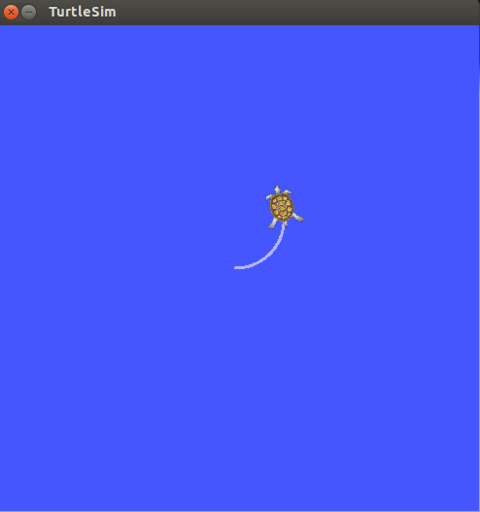
\includegraphics[width=\columnwidth]{pictures/chapter4/pic_04_02.png}
  \caption{配信したメッセージが反映された様子}
\end{figure}

なお、メッセージ型の詳細は、以下のように「rosmsg show [メッセージ名]」で調べることができる。

\begin{lstlisting}[language=ROS]
$ rosmsg show geometry_msgs/Twist
geometry_msgs/Vector3 linear
float64 x
float64 y
float64 z
geometry_msgs/Vector3 angular
float64 x
float64 y
float64 z
\end{lstlisting}

\begin{exercise}[ROSで使用される単位]
単位(unit)はROS規則で取決められており、パッケージ作成時にhttp://www.ros.org/reps/rep-0103.htmlで確認する必要がある。上の例の速度の場合、meter/secやradian/secを使用している。
\end{exercise}


%-------------------------------------------------------------------------------
\subsection{rosservice:ROSサービス情報の確認}

rosserviceは、ROSサービスの情報を確認するためのコマンドである。

\begin{itemize}
\item rosservice [オプション]
\end{itemize}

オプションには、list、info、type、find、uri、args、callなどが指定できる。

rosserviceコマンドの例を示す前に、一度すべてのノードを終了する。次に、それぞれ別のターミナルウィンドウで、次のコマンドを実行して、turtlesim\_nodeとturtle\_teleop\_keyを実行する。

\begin{lstlisting}[language=ROS]
$ roscore
\end{lstlisting}

\begin{lstlisting}[language=ROS]
$ rosrun turtlesim turtlesim_node
\end{lstlisting}

\begin{lstlisting}[language=ROS]
$ rosrun turtlesim turtle_teleop_key
\end{lstlisting}

%-------------------------------------------------------------------------------
\subsubsection{rosservice list:アクティブなサービスの一覧を表示}

rosservice listは使用中のサービスの一覧を表示するコマンドである。

\begin{lstlisting}[language=ROS]
$ rosservice list
/clear
/kill
/reset
/rosout/get_loggers
/rosout/set_logger_level
/spawn
/teleop_turtle/get_loggers
/teleop_turtle/set_logger_level
/turtle1/set_pen
/turtle1/teleport_absolute
/turtle1/teleport_relative
/turtlesim/get_loggers
/turtlesim/set_logger_level
\end{lstlisting}

%-------------------------------------------------------------------------------
\subsubsection{rosservice info [サービス名]:指定されたサービスの情報を表示}

rosservice infoは、実行ノードやPC名、サービス型など、指定されたサービスの詳細な情報を表示するコマンドである。下の例では、/turtle1/set\_penサービスのノード名、URI、サービス型、パラメータを確認できる。

\begin{lstlisting}[language=ROS]
$ rosservice info /turtle1/set_pen
Node: /turtlesim
URI: rosrpc://192.168.4.100:34715
Type: turtlesim/SetPen
Args: r g b width off
\end{lstlisting}

%-------------------------------------------------------------------------------
\subsubsection{rosservice type [サービス名]:指定されたサービスのサービス型を表示}

rosservice typeは、指定したサービスで使用しているサービス型を表示するコマンドである。次の例では、/turtle1/set\_penサービスで使用しているサービスの型がturtlesim/SetPenであることが確認できる。

\begin{lstlisting}[language=ROS]
$ rosservice type /turtle1/set_pen
turtlesim/SetPen
\end{lstlisting}

%-------------------------------------------------------------------------------
\subsubsection{rosservice find [サービス型]:指定したサービス型を使用しているサービスを検索}

rosservice findは指定したサービス型を使用しているサービスを検索し、表示するコマンドである。下の例では、turtlesim/SetPen型を持つサービスが表示されている。

\begin{lstlisting}[language=ROS]
$ rosservice find turtlesim/SetPen
/turtle1/set_pen
\end{lstlisting}

%-------------------------------------------------------------------------------
\subsubsection{rosservice uri [サービス名]:指定されたサービスのROSRPC URIの表示}

rosservice uriは指定したサービスのURIを表示するコマンドである。下の例は、/turtle1/set\_penサービスのROSRPC URIを表示している。

\begin{lstlisting}[language=ROS]
$ rosservice uri /turtle1/set_pen
URI: rosrpc://192.168.4.100:34715
\end{lstlisting}

%-------------------------------------------------------------------------------
\subsubsection{rosservice args [サービス名]:サービスパラメータの表示}

rosservice argsは指定したサービスのパラメータを表示するコマンドである。下の例は、/turtle1/set\_penサービスの各パラメータを表示している様子でありr、g、b、width、offというパラメータが使用されていることが確認できる。

\begin{lstlisting}[language=ROS]
$ rosservice args /turtle1/set_pen
r g b width off
\end{lstlisting}

%-------------------------------------------------------------------------------
\subsubsection{rosservice call [サービス名] [パラメータ]:指定されたサービスのリクエストを実行}

rosservice callは、コマンドラインから指定されたサービスをリクエストするコマンドである。サービスのテストのために使用される便利なコマンドであり、使用頻度は高い。次の例は、/turtle1/set\_penサービスへリクエストするものである。使用された「255 0 0 5 0」の5つの数値はそれぞれ/turtle1/set\_penサービスに使用されているパラメータ(r、g、b、width、off)に対応する。赤を表すrは最大値の255を、g、bはいずれも0とし、widthは5の太さを設定、線の可視化を表すoffは0(false)と設定している。

\begin{lstlisting}[language=ROS]
$ rosservice call /turtle1/set_pen 255 0 0 5 0
\end{lstlisting}

上のコマンドでサービスをリクエストすることで、turtlesimに使用されるペンの特性を変えられる。turtle\_teleop\_keyコマンドで移動した結果、次のように白いペンの色が赤で表示されることが確認できる。

\begin{figure}[h]
  \centering
  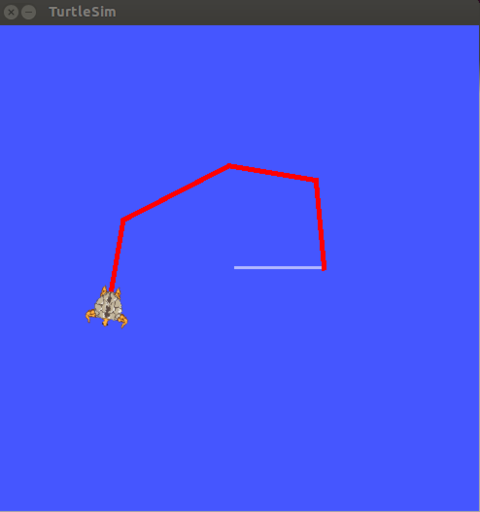
\includegraphics[width=\columnwidth]{pictures/chapter4/pic_04_03.png}
  \caption{rosservice callの例}
\end{figure}

%-------------------------------------------------------------------------------
\subsubsection{rosparam:ROSパラメータ情報の確認と修正}

rosparamは、ROSサービスのパラメータの情報の確認するためのコマンドである。

\begin{itemize}
\item rosparam [オプション]
\end{itemize}

オプションには、list、get、set、dump、load、deleteなどが指定できる。

rosparamコマンドの例を実行する前に、一度すべてのノードを終了する。次に、それぞれ別のターミナルウィンドウで、次のコマンドを実行して、turtlesim\_nodeとturtle\_teleop\_keyを実行する。

\begin{lstlisting}[language=ROS]
$ roscore
\end{lstlisting}

\begin{lstlisting}[language=ROS]
$ rosrun turtlesim turtlesim_node
\end{lstlisting}

\begin{lstlisting}[language=ROS]
$ rosrun turtlesim turtle_teleop_key
\end{lstlisting}

%-------------------------------------------------------------------------------
\subsubsection{rosparam list:パラメータの一覧の表示}

rosparam listは使用中のパラメータの一覧を表示するコマンドである。

\begin{lstlisting}[language=ROS]
$ rosparam list
/background_b
/background_g
/background_r
/rosdistro
/roslaunch/uris/host_192_168_4_100  39536
/rosversion
/run_id
\end{lstlisting}

%-------------------------------------------------------------------------------
\subsubsection{rosparam get [パラメータ名]:パラメータ値の読み込み}

rosparam getは指定したパラメータの値を表示するコマンドである。次の例では、/background\_bパラメータの値を確認できる。

\begin{lstlisting}[language=ROS]
$ rosparam get /background_b
255
\end{lstlisting}

特定のパラメータではなく、すべてのパラメータの値を確認したいときには、オプションで「/」を指定する。

\begin{lstlisting}[language=ROS]
$ rosparam get /
background_b: 255
background_g: 86
background_r: 69
rosdistro: 'indigo'
roslaunch: uris: {host_192_168_4_100  39536: 'http://192.168.4.100:39536/'} rosversion: '1.11.10'
run_id: 93598bxx.44xx.11xx.a0xx.d43d7e97xxxx
\end{lstlisting}

%-------------------------------------------------------------------------------
\subsubsection{rosparam dump [ファイル名]:パラメータ値を指定したファイルに保存}

rosparam dumpは、現在のすべてのパラメータ値を指定したファイルに保存するコマンドである。下の例では、現在のパラメータ値をparameters.yamlのファイルに保存している。毎回使用されるパラメータの値を保存しておき、rosparam loadコマンドで呼び出すことにより、以降の実行時に繰り返し使用できる。

\begin{lstlisting}[language=ROS]
$ rosparam dump ~/parameters.yaml
\end{lstlisting}

%-------------------------------------------------------------------------------
\subsubsection{rosparam set [パラメータ名]:パラメータ値の書き込み}

rosparam dumpは、指定したパラメータに値を設定するコマンドである。下の例では、turtlesimノードの背景色に関するパラメータであるbackground\_bを0に設定している。

\begin{lstlisting}[language=ROS]
$ rosparam set background_b 0
$ rosservice call clear
\end{lstlisting}

これにより、RGBは255、86、69から0、86、69に変更されるため、図4-4の右図のように背景色が濃い緑になる。ただし、turtlesimノードの仕様により、変更を反映するためには、「rosparam set background\_b0」コマンドでパラメータを変更した後、「rosservice call clear」コマンドで画面を更新する必要がある。

\begin{figure}[h]
  \centering
  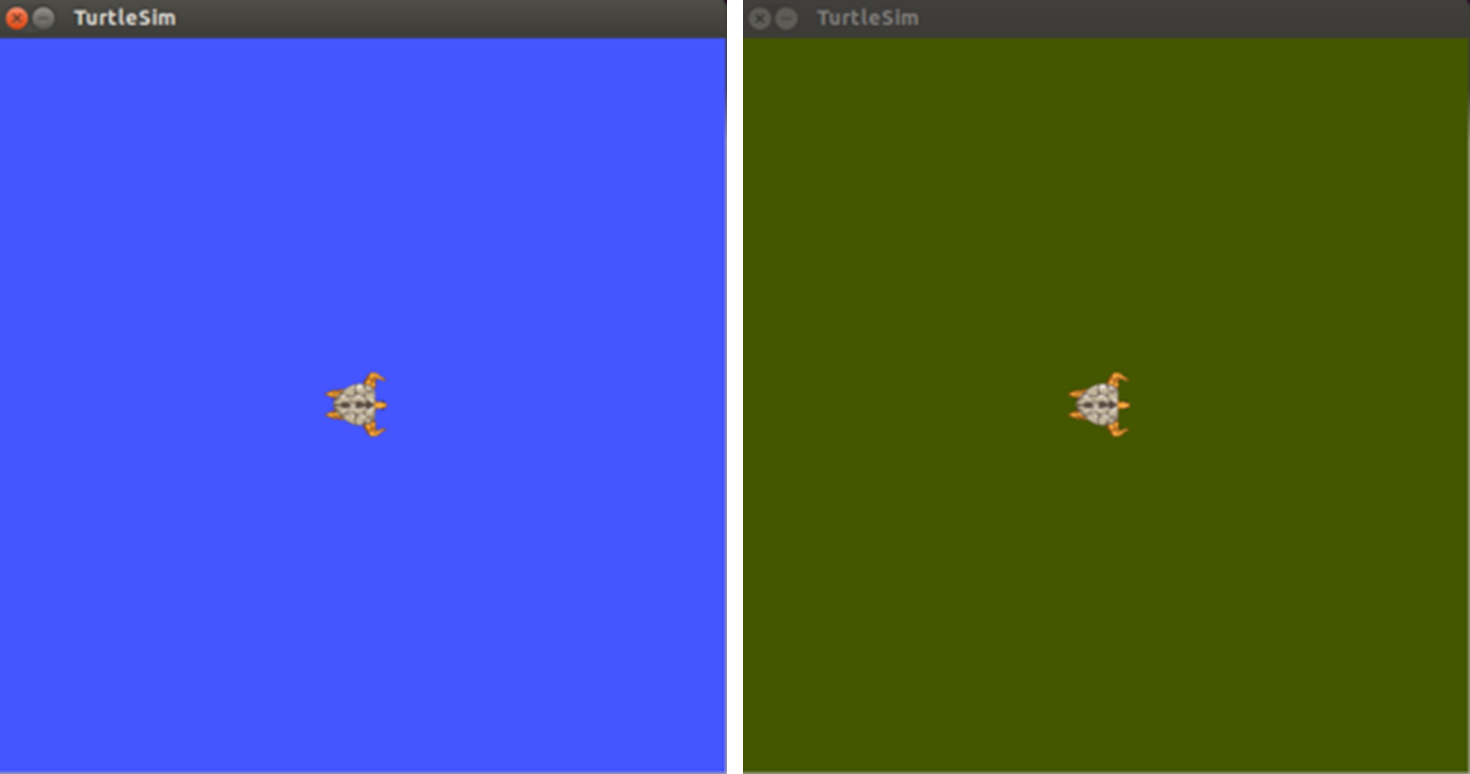
\includegraphics[width=\columnwidth]{pictures/chapter4/pic_04_04.png}
  \caption{rosparam setの例}
\end{figure}

%-------------------------------------------------------------------------------
\subsubsection{rosparam load [ファイル名]:指定したファイルに保存されたパラメータの読み込み}

rospasm loadは、指定したファイルから保存されたパラメータを読み込むコマンドであり、頻繁に使用される。下の例では、「rosparam dump」コマンドとは逆に、parameters.yamlファイルを読み込み、現在のパラメータ値として使用している。このコマンドの後、「rosservice call clear」コマンドを実行し、取得したファイルのパラメータ値を適用する。図4-4で緑になった背景が、「rosparam dump」コマンド実行前の青色の背景に戻ることが分かる。

\begin{lstlisting}[language=ROS]
$ rosparam load ~/parameters.yaml
$ rosservice call clear
\end{lstlisting}

%-------------------------------------------------------------------------------
\subsubsection{rosparam delete [パラメータ名]:パラメータを削除}

rosparam deleteは、指定したパラメータを削除するコマンドである。削除されたパラメータは、rosparam listコマンドで表示されず、パラメータの値は規定値に戻る。

\begin{lstlisting}[language=ROS]
$ rosparam delete /background_b
\end{lstlisting}

%-------------------------------------------------------------------------------
\subsection{rosmsg:ROSメッセージ情報の確認}

rosmsgは、ROSメッセージの情報の確認するためのコマンドである。

\begin{itemize}
\item   rosmsg [オプション]
\end{itemize}

オプションには、list、show、md5、package、packagesなどが指定できる。

rosmsg コマンドの例を示す前に、一度すべてのノードを終了する。次に、それぞれ別のターミナルウィンドウで、次のコマンドを実行して、turtlesim\_nodeとturtle\_teleop\_keyを実行する。

\begin{lstlisting}[language=ROS]
$ roscore
\end{lstlisting}

\begin{lstlisting}[language=ROS]
$ rosrun turtlesim turtlesim_node
\end{lstlisting}

\begin{lstlisting}[language=ROS]
$ rosrun turtlesim turtle_teleop_key
\end{lstlisting}

%-------------------------------------------------------------------------------
\subsubsection{rosmsg list:すべてのメッセージの一覧を表示}

rosmsg listは、インストール済みパッケージのすべてのメッセージを表示するコマンドである。

\begin{lstlisting}[language=ROS]
$ rosmsg list
actionlib/TestAction
actionlib/TestActionFeedback
actionlib/TestActionGoal
actionlib/TestActionResult
actionlib/TestFeedback
actionlib/TestGoal
sensor_msgs/Joy
sensor_msgs/JoyFeedback
sensor_msgs/JoyFeedbackArray
sensor_msgs/LaserEcho
zeroconf_msgs/DiscoveredService
%*〜省略〜*)
\end{lstlisting}

%-------------------------------------------------------------------------------
\subsubsection{rosmsg show [メッセージ名]:指定したメッセージのメッセージ型を表示}

rosmsg showは、指定したメッセージのメッセージ型を表示するコマンドである。下の例では、turtlesim/Poseメッセージのメッセージ型を出力している様子である。float32(浮動小数点型変数)で、x、y、theta、linear\_velocity、angular\_velocityの5つの変数からなるメッセージであることが確認できる。

\begin{lstlisting}[language=ROS]
$ rosmsg show turtlesim/Pose
float32 x
float32 y
float32 theta
float32 linear_velocity
float32 angular_velocity
\end{lstlisting}

%-------------------------------------------------------------------------------
\subsubsection{rosmsg md5 [メッセージ名]:指定したメッセージのmd5sumを表示}

rosmsg md5は、指定したメッセージのmd5sumの値を表示するコマンドである。下の例は、turtlesim/Poseメッセージのmd5sumの値を確認している様子である。メッセージ通信中にMD5問題が発生し、md5sumを確認する必要がある時、使用される。

\begin{lstlisting}[language=ROS]
$ rosmsg md5 turtlesim/Pose
863b248d5016ca62ea2e895ae5265cf9
\end{lstlisting}

%-------------------------------------------------------------------------------
\subsubsection{rosmsg package [パッケージ名]:指定したパッケージで使用されるメッセージの一覧を表示}

rosmsg packageは、指定したパッケージで使用されるメッセージを表示するコマンドである。

\begin{lstlisting}[language=ROS]
$ rosmsg package turtlesim
turtlesim/Color
turtlesim/Pose
\end{lstlisting}

%-------------------------------------------------------------------------------
\subsubsection{rosmsg packages:メッセージを使用しているすべてのパッケージの一覧を表示}

rosmsg packagesは、メッセージを使用しているすべてのパッケージを表示するコマンドである。

\begin{lstlisting}[language=ROS]
$ rosmsg packages
actionlib
actionlib_msgs
actionlib_tutorials
base_local_planner
bond
control_msgs costmap_2d
%*〜省略〜*)
\end{lstlisting}

%-------------------------------------------------------------------------------
\subsection{rossrv:ROSサービス情報の確認}

rossrvは、ROSサービスの情報の確認するためのコマンドである。

\begin{itemize}
\item rossrv [オプション]
\end{itemize}

オプションには、rosmsgと同様に、list、show、md5、package、packagesなどが指定できる。

rossrvコマンドの例を示す前に、一度すべてのノードを終了する。次に、それぞれ別のターミナルウィンドウで、次のコマンドを実行して、turtlesim\_nodeとturtle\_teleop\_keyを実行する。

\begin{lstlisting}[language=ROS]
$ roscore
\end{lstlisting}

\begin{lstlisting}[language=ROS]
$ rosrun turtlesim turtlesim_node
\end{lstlisting}

\begin{lstlisting}[language=ROS]
$ rosrun turtlesim turtle_teleop_key
\end{lstlisting}


%-------------------------------------------------------------------------------
\subsubsection{rossrv list:すべてのサービスの一覧を表示}

rossrv listは、インストール済みパッケージのすべてのサービスを表示するコマンドである。

\begin{lstlisting}[language=ROS]
$ rossrv list
control_msgs/QueryCalibrationState
control_msgs/QueryTrajectoryState
diagnostic_msgs/SelfTest
dynamic_reconfigure/Reconfigure
gazebo_msgs/ApplyBodyWrench
gazebo_msgs/ApplyJointEffort
gazebo_msgs/BodyRequest
gazebo_msgs/DeleteModel
%*〜省略〜*)
\end{lstlisting}

%-------------------------------------------------------------------------------
\subsubsection{rossrv show [サービス名]:指定されたサービスの情報を表示}

rossrv showは、指定したサービスの情報を表示するコマンドである。下の例では、turtlesim/SetPenサービスの情報を出力した例である。uint8(符号なし8ビット整数型変数)でr、g、b、width、offの5つの変数が含まれていることが確認できる。参考までに「---」は、サービスファイルのリクエストとレスポンスを区分する線として使用され、このturtlesim/SetPenサービスはリクエストだけがあり、レスポンスに該当するものがないことが分かる。この部分については、6.3節で詳細に取り上げる。

\begin{lstlisting}[language=ROS]
$ rossrv show turtlesim/SetPen
uint8 r
uint8 g
uint8 b
uint8 width
uint8 off
---
\end{lstlisting}

%-------------------------------------------------------------------------------
\subsubsection{rossrv md5 [サービス名]:指定されたサービスのmd5sumを表示}

rossrv md5は、指定したサービスのmd5sumの値を表示するコマンドである。下の例は、turtlesim/SetPenサービスのmd5sum情報を確認している例である。サービスの使用中にMD5問題が発生した場合、md5sumを確認する必要がある時、使用されるコマンドである。

\begin{lstlisting}[language=ROS]
$ rossrv md5 turtlesim/SetPen
9f452acce566bf0c0954594f69a8e41b
\end{lstlisting}

%-------------------------------------------------------------------------------
\subsubsection{rossrv package [パッケージ名]:指定したパッケージで使用しているサービスの一覧を表示}

rossrv packageは、指定したパッケージで使用されるサービスを表示するコマンドである。

\begin{lstlisting}[language=ROS]
$ rossrv package turtlesim
turtlesim/Kill
turtlesim/SetPen
turtlesim/Spawn
turtlesim/TeleportAbsolute
turtlesim/TeleportRelative
\end{lstlisting}

%-------------------------------------------------------------------------------
\subsubsection{rossrv packages:サービスを使用しているすべてのパッケージの一覧を表示}

rossrv packagesは、サービスを使用しているすべてのパッケージを表示するコマンドである。

\begin{lstlisting}[language=ROS]
$ rossrv packages
control_msgs
diagnostic_msgs
dynamic_reconfigure
gazebo_msgs
map_msgs
nav_msgs
navfn nodelet
roscpp sensor_msgs
std_srvs
tf
tf2_msgs
turtlesim
%*〜省略〜*)
\end{lstlisting}

%-------------------------------------------------------------------------------
\subsection{rosbag:ROSメッセージの記録と再生}

ros bagは、ROSメッセージを記録、再生するためのコマンドである。ROSは、bagという形式でメッセージを保存し、必要なときに再生して、記録した時の状況をそのまま再現できる。

\begin{itemize}
\item rosbag [オプション]
\end{itemize}

オプションには、record、info、play、compress、decompress、filter、reindex bag、check bag、fixなどが指定できる。

rosbagコマンドの例を示す前に、一度すべてのノードを終了する。次に、それぞれ別のターミナルウィンドウで、次のコマンドを実行して、turtlesim\_nodeとturtle\_teleop\_keyを実行する。

\begin{lstlisting}[language=ROS]
$ roscore
\end{lstlisting}

\begin{lstlisting}[language=ROS]
$ rosrun turtlesim turtlesim_node
\end{lstlisting}

\begin{lstlisting}[language=ROS]
$ rosrun turtlesim turtle_teleop_key
\end{lstlisting}


%-------------------------------------------------------------------------------
\subsubsection{rosbag record [オプション] [トピック名]:指定されたトピックのメッセージをbagファイルに記録}

rosbag recordは、すべてのトピック、あるいは指定したトピックのメッセージをファイルに記録するコマンドである。
まず、rostopic listコマンドを使用し、使用されているトピックを確認する。

\begin{lstlisting}[language=ROS]
$ rostopic list
/rosout
/rosout_agg
/turtle1/cmd_vel
/turtle1/color_sensor
/turtle1/pose
\end{lstlisting}

次に、使用しているトピックの中から、記録するトピックとして/turtle1/cmd\_velトピックを指定し、bagの記録を開始する。この際、「-O」のオプションで保存ファイル名を指定できる。下の例ではmsglog.bagに保存する。その後、turtle_teleop_keyノードでキーボードの矢印キーで亀を移動させると、オプションで指定された/turtle1/cmd\_velトピックが記録される。また、<Ctrl>+<C>を押して記録を終了すると、以下のようにmsglog.bagファイルが生成される。

\begin{lstlisting}[language=ROS]
$ rosbag record -O msglog.bag /turtle1/cmd_vel
[INFO] [1423029313.526437636]: Subscribing to /turtle1/cmd_vel
[INFO] [1423029313.534906460]: Recording to msglog.bag.
\end{lstlisting}

特定のトピックではなく、すべてのトピックを同時に記録したい場合は、以下のようにオプションの「-a」を付ける。

\begin{lstlisting}[language=ROS]
$ rosbag record -a -O msglog.bag
[INFO] [1423029391.499585832]: Recording to msglog.bag.
[INFO] [1423029391.500622809]: Subscribing to /turtle1/color_sensor
[INFO] [1423029391.507350765]: Subscribing to /turtle1/cmd_vel
[INFO] [1423029391.514320943]: Subscribing to /rosout
[INFO] [1423029391.528439120]: Subscribing to /rosout_agg
[INFO] [1423029391.547867201]: Subscribing to /turtle1/pose
\end{lstlisting}

%-------------------------------------------------------------------------------
\subsubsection{rosbag info [ファイル名]:bagファイルの情報を確認}

rosbag infoは、記録したbagファイルの情報を表示するコマンドである。下の例では、記録した/turtle1/cmd\_velトピックのbagファイルが、合計167個のメッセージの記録で構成されていることや、使用されたメッセージの型、パス、バージョン、記録時間などの情報が確認できる。

\begin{lstlisting}[language=ROS]
$ rosbag info msglog.bag
path: msglog.bag
version: 2.0
duration: 12.7s
start: Feb 04 2015 14:55:15.33 (1423029315.33)
end: Feb 04 2015 14:55:28.04 (1423029328.04)
size: 22.5 KB
messages: 167
compression: none [1/1 chunks]
types: geometry_msgs/Twist [9f195f881246fdfa2798d1d3eebca84a]
topics: /turtle1/cmd_vel
167 msgs : geometry_msgs/Twist
\end{lstlisting}

%-------------------------------------------------------------------------------
\subsubsection{rosbag play [ファイル名]:指定されたbagファイルを再生}

rosbag playは、記録したbagファイルを再生するコマンドである。下の例は、上のrosbag recordコマンドの説明で記録したmsglog.bagを再生したものであり、記録時の/turtle1/cmd\_velメッセージがそのまま再生され、画面上のカメが動く様子を確認できる。ただし、turtlesim\_nodeを再起動し、ロボット軌跡とロボットの位置を初期化する必要がある。問題なければ、図4-5のように、rosbag recordで記録した時と同じ軌跡を得ることができる。

\begin{lstlisting}[language=ROS]
$ rosbag play msglog.bag
[INFO] [1423029542.171454338]: Opening msglog.bag
Waiting 0.2 seconds after advertising topics... done.
Hit space to toggle paused, or 's' to step.
[RUNNING]  Bag Time: 1423029315.327811  Duration: 0.000000 / 12.713
[RUNNING]  Bag Time: 1423029315.327889  Duration: 0.000078 / 12.713
%*〜省略〜*)
\end{lstlisting}

\begin{figure}[h]
  \centering
  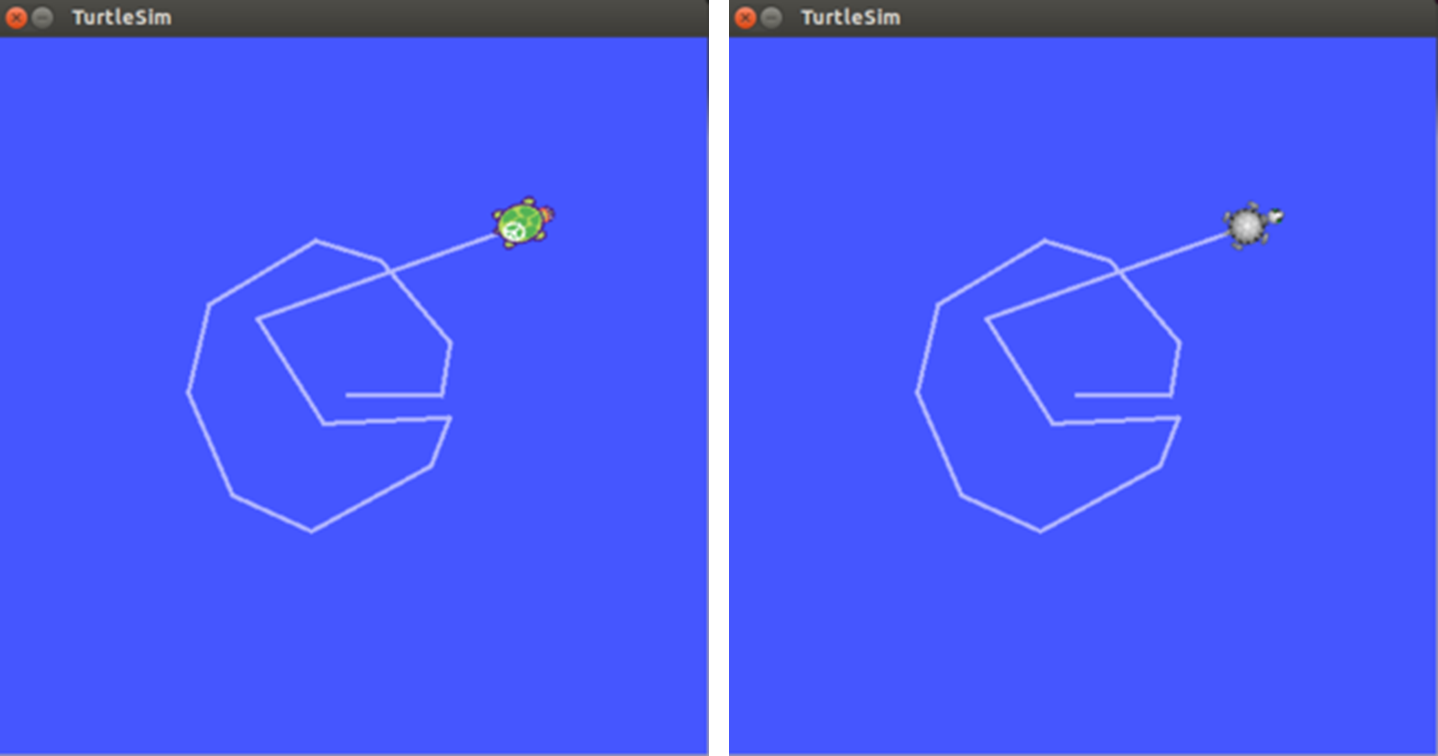
\includegraphics[width=\columnwidth]{pictures/chapter4/pic_04_05.png}
  \caption{rosbag playの例(左:記録時、右:再生時)}
\end{figure}

%-------------------------------------------------------------------------------
\subsubsection{rosbag compress [ファイル名]:指定されたbagファイルを圧縮}

rosbag compressは、記録したbagファイルを圧縮するコマンドである。bagファイルに長時間記録すると、bagファイルのサーズが大きくなる。そこで、rosbag compressコマンドでbagファイルを圧縮して、ファイルサイズを小さくできる。

\begin{lstlisting}[language=ROS]
$ rosbag compress msglog.bag
msglog.bag  100%   15.8 KB 00:00
\end{lstlisting}

上の例では、bagファイルが次のように3分の1に縮小される。圧縮前の元ファイルは、origという拡張子が追加され、別に保存されている。

\begin{lstlisting}[language=ROS]
msglog.bag 8.5kB
msglog.orig.bag 23.0kB
\end{lstlisting}

%-------------------------------------------------------------------------------
\subsubsection{rosbag decompress [ファイル名]:指定されたbagファイルを圧縮解除}

rosbag decompressは、rosbag compressコマンドで圧縮されたファイルを圧縮前の状態に戻すコマンドである。

\begin{lstlisting}[language=ROS]
$ rosbag decompress msglog.bag
msglog.bag  100%  15.8 KB 00:00
\end{lstlisting}

%-------------------------------------------------------------------------------
\subsubsection{rosbag filter [入力ファイル] [出力ファイル] [オプション]:bagファイルの再作成}

rosbag filterは、作成済みのbagファイルから、指定されたトピックのみを残して、新しいbagファイルを作成するコマンドである。

rosbag filterコマンドの例を実行する前に、一度すべてのノードを終了する。次に、それぞれ別のターミナルウィンドウで、次のコマンドを実行して、turtlesim\_nodeとturtle\_teleop\_keyを実行する。

\begin{lstlisting}[language=ROS]
$ roscore
\end{lstlisting}

\begin{lstlisting}[language=ROS]
$ rosrun turtlesim turtlesim_node
\end{lstlisting}

\begin{lstlisting}[language=ROS]
$ rosrun turtlesim turtle_teleop_key
\end{lstlisting}

次に、rosbag recordコマンドを実行し、msglog.bagファイルに全てのトピックを記録する。

\begin{lstlisting}[language=ROS]
$ rosbag record -O msglog.bag -a
\end{lstlisting}

turtle\_teleop\_keyを実行したターミナルで矢印キーを操作し、亀を移動させる。その後、<Ctrol>+<C>でrosbag recordコマンドを終了する。

記録したmsglog.bagをrosbag infoコマンドで確認すると、以下のように/rosout, /turtle1/cmd\_vel, /turtle1/color\_sensor, /turtle1/pose トピックが記録されていることがわかる。

\begin{lstlisting}[language=ROS]
$ rosbag info msglog.bag
path:        msglog.bag
version:     2.0
duration:    12.6s
start:       Jul 16 2015 19:08:28.26 (1437041308.26)
end:         Jul 16 2015 19:08:40.88 (1437041320.88)
size:        127.6 KB
messages:    1645
compression: none [1/1 chunks]
types:       geometry_msgs/Twist [9f195f881246fdfa2798d1d3eebca84a]
             rosgraph_msgs/Log   [acffd30cd6b6de30f120938c17c593fb]
             turtlesim/Color     [353891e354491c51aabe32df673fb446]
             turtlesim/Pose      [863b248d5016ca62ea2e895ae5265cf9]
topics:      /rosout                   4 msgs    : rosgraph_msgs/Log   (2 connections)
             /turtle1/cmd_vel         92 msgs    : geometry_msgs/Twist
             /turtle1/color_sensor   775 msgs    : turtlesim/Color
             /turtle1/pose           774 msgs    : turtlesim/Pose
\end{lstlisting}

次に、rosbag filterコマンドにより、/turtle1/cmd\_velトピックのみを残して、他のトピックを削除する。以下では、出力ファイルをonly\_cmd\_vel.bagとしている。

\begin{lstlisting}[language=ROS]
$ rosbag filter msglog.bag only_cmd_vel.bag "topic == '/turtle1/cmd_vel'"
\end{lstlisting}

rosbag infoコマンドによりonly\_cmd\_vel.bagファイルを確認すると、/turtle1/cmd\_velトピックのみが含まれていることがわかる。このようにrosbag filterコマンドは、指定されたトピックのみを残して、新しいbagファイルを作成するために使用される。

\begin{lstlisting}[language=ROS]
$ rosbag info only_cmd_vel.bag
path:    only_cmd_vel.bag
version: 2.0
size:    4.0 KB
rt@rt:~$ rosbag info only_cmd_vel.bag
path:        only_cmd_vel.bag
version:     2.0
duration:    5.9s
start:       Jul 16 2015 19:08:32.09 (1437041312.09)
end:         Jul 16 2015 19:08:38.03 (1437041318.03)
size:        14.7 KB
messages:    92
compression: none [1/1 chunks]
types:       geometry_msgs/Twist [9f195f881246fdfa2798d1d3eebca84a]
topics:      /turtle1/cmd_vel   92 msgs    : geometry_msgs/Twist
\end{lstlisting}

複数のトピックを残す場合は、以下のようにトピック名を続けて指定する。

\begin{lstlisting}[language=ROS]
$ rosbag filter msglog.bag only_cmd_vel.bag "topic == '/turtle1/cmd_vel' or topic == '/turtle1/pose'"
\end{lstlisting}

%-------------------------------------------------------------------------------
\subsubsection{rosbag reindex [ファイル名]:bagファイルの再インデックス}

rosbag reindex は、bagファイルに問題があり再生できない場合、再インデックスによりbagファイルを修復するコマンドである。元のbagファイルはmsglog.orig.bagとして保存され、修復されたbagファイルは同じ名前で上書きされる。

\begin{lstlisting}[language=ROS]
$ rosbag reindex msglog.bag
 msglog.bag                       100%            123.8 KB 00:00
\end{lstlisting}

%-------------------------------------------------------------------------------
\subsubsection{rosbag check bag [ファイル名]:bagファイルの再生確認}

rosbag check bagは、指定されたbagファイルが現在のROSシステムで再生できるかを確認するコマンドである。現在のROSシステムで再生できる場合、以下のように表示される。

\begin{lstlisting}[language=ROS]
$ rosbag check msglog.bag
Bag file is up to date.
\end{lstlisting}

%-------------------------------------------------------------------------------
\subsubsection{rosbag fix [入力ファイル] [出力ファイル] [オプション]:bagファイルのバージョン変更}

rosbag fixは、ROSのバージョンが異なり現在のROSシステムでは再生が不可能なbagファイルを、再生できる形式に変換するコマンドである。

\begin{lstlisting}[language=ROS]
$ rosbag fix msglog.bag repaired_msglog.bag
Bag migrated successfully.
\end{lstlisting}

%-------------------------------------------------------------------------------
\section{ROS catkinコマンド}\index{ROS catkinコマンド}

ROS catkinは、catkinビルドシステムを用いてパッケージをビルドする際に使用される。

\vspace{\baselineskip}
\noindent
\begin{description}
\item[catkin\_create_pkg](★★★):catkinビルドシステムでパッケージを自動生成
\item[catkin\_make](★★★):catkinビルドシステムのビルド命令
\item[catkin\_eclipse](★★☆):catkinビルドシステムで生成したパッケージをEclipseで使用できるように変更
\item[catkin\_prepare\_release](★★☆):リリース準備するときに使用されるchangelog整理とバージョンのタグ管理
\item[catkin\_generate\_changelog](★★☆):リリースするときCHANGELOG.rstファイルの作成又は更新
\item[catkin\_init\_workspace](★☆☆):catkinビルドシステムの作業フォルダの初期化
\item[catkin\_find](☆☆☆):catkin検索
\end{description}

%-------------------------------------------------------------------------------
\subsection{catkin\_create\_pkg:catkinビルドシステムでパッケージを自動生成}

catkin\_create\_pkgはCMakeLists.txtとpackage.xmlを含む空のパッケージを生成するコマンドである。詳しい使用方法は3.4.1項を参照のこと。

\begin{itemize}
\item catkin\_create\_pkg <パッケージ名> [依存パッケージ1] [依存パッケージ2] …
\end{itemize}

catkin\_create\_pkgの使用例を下に示す。

\begin{lstlisting}[language=ROS]
$ catkin_create_pkg my_package roscpp std_msgs
\end{lstlisting}

%-------------------------------------------------------------------------------
\subsection{catkin\_make:catkinビルドシステムのビルド命令}

catkin\_makeはユーザーが作成したパッケージまたはダウンロードしたパッケージをビルドするコマンドである。

\begin{itemize}
\item  catkin\_make
\end{itemize}

~/catkin\_ws/srcフォルダにある全てのパッケージをビルドする例を示す。

\begin{lstlisting}[language=ROS]
$ cd ~/catkin_ws
$ catkin_make
\end{lstlisting}

全てのパッケージではなく、一部のパッケージのみビルドする場合は、以下ように--pkg [パッケージ名] オプションを指定して実行する。

\begin{lstlisting}[language=ROS]
catkin_make --pkg user_ros_tutorials
\end{lstlisting}

%-------------------------------------------------------------------------------
\subsection{catkin\_eclipse:Eclipseを使用したパッケージの管理}

catkin\_eclipseは、統合開発環境(IDE)の一つであるEclipseを用いて、ユーザーが作成したパッケージを管理し、プログラミングを行う環境を構築するコマンドである。

\begin{itemize}
\item catkin\_eclipse
\end{itemize}

このコマンドを実行すると~/catkin\_ws/build/.cproject、~/catkin\_ws/build/.projectなど、Eclipse用のプロジェクトファイルが生成される。Eclipse のメニューから「Makefile Project with Existing Code」を選択し、「~/catkin\_ws/build/」を選択すると、~/catkin\_ws/srcにある全パッケージをEclipseで管理できる。

\begin{lstlisting}[language=ROS]
$ cd ~/catkin_ws
$ catkin_eclipse
\end{lstlisting}

%-------------------------------------------------------------------------------
\subsection{catkin\_generate\_changelog:CHANGELOG.rstファイルの作成}

catkin\_generate\_changelogは、パッケージのバージョンアップ時に変更点を記述するCHANGELOG.rstファイルを作成するコマンドである。

\begin{itemize}
\item catkin\_generate\_changelog
\end{itemize}

%-------------------------------------------------------------------------------
\subsection{catkin\_prepare\_release:リリース準備するときに使用されるchangelog整理とバージョンのタグ管理}

catkin\_prepare\_releaseは、catkin\_generate\_changelogコマンドで作成されたCHANGELOG.rstを更新するとき使用されるコマンドである。

\begin{itemize}
\item catkin\_prepare\_release
\end{itemize}

catkin\_generate\_changelogとcatkin\_prepare\_releaseコマンドは、作成したパッケージをROSレポジトリ注3に登録する時や、登録されたパッケージのバージョンアップの際に使用されるコマンドである。

%-------------------------------------------------------------------------------
\subsection{catkin\_init\_workspace:catkinビルドシステムの作業フォルダの初期化}

catkin\_init\_workspaceはユーザーの作業フォルダ(~/catkin\_ws/src)の初期化コマンドである。

\begin{itemize}
\item catkin\_init\_workspace
\end{itemize}

2.1.1項で説明したように、このコマンドはROSインストールの後に一度だけ行えばよい。

\begin{lstlisting}[language=ROS]
$ cd ~/catkin_ws/src
$ catkin_init_workspace
\end{lstlisting}

%-------------------------------------------------------------------------------
\subsection{catkin\_find:ワークスペースの検索}

catkin\_findはプロジェクト毎に作業フォルダを表示するコマンドである。

\begin{itemize}
\item  catkin\_find [パッケージ名]
\end{itemize}

catkin\_findコマンドを実行すると、使用している全ての作業フォルダを調べることができる。また、「catkin\_find パッケージ名」とすると、オプションで指定したパッケージに関連する作業フォルダが表示される。

\begin{lstlisting}[language=ROS]
$ catkin_find
/home/rt/catkin_ws/devel/include
/home/rt/catkin_ws/devel/lib
/home/rt/catkin_ws/devel/share
/opt/ros/indigo/bin
/opt/ros/indigo/etc
/opt/ros/indigo/include
/opt/ros/indigo/lib
/opt/ros/indigo/share
\end{lstlisting}

\begin{lstlisting}[language=ROS]
$ catkin_find turtlesim
/opt/ros/indigo/include/turtlesim
/opt/ros/indigo/lib/turtlesim
/opt/ros/indigo/share/turtlesim
\end{lstlisting}

%-------------------------------------------------------------------------------
\section{ROSパッケージコマンド}\index{ROSパッケージコマンド}
ROS パッケージは、パッケージの情報表示や関連パッケージのインストールなど、ROSのパッケージ操作に使用される。

\vspace{\baselineskip}
\noindent
\begin{description}
\item[rospack](★★☆)ros+pack(age):指定したROSパッケージに関連する情報を表示
\item[rosinstall](★☆☆)ros+install:ROS追加パッケージの自動インストール
\item[rosdep](★☆☆)ros+dep(endencies):ROSパッケージの依存関係ファイルのインストール
\item[roslocate](☆☆☆)ros+locate:ROSパッケージの情報表示
\item[roscreate-pkg](☆☆☆)ros+create-pkg:ROSパッケージの自動生成(旧rosbuildシステムで使用)
\item[rosmake](☆☆☆)ros+make:ROSパッケージをビルド(旧rosbuildシステムで使用)
\end{description}

%-------------------------------------------------------------------------------
\subsection{rospack:指定したROSパッケージに関連する情報を表示}

rospackは指定したROSパッケージに関連する保存先、依存関係、全パッケージのリストなどの情報を表示するコマンドである。

\begin{itemize}
\item  rospack [オプション] [パッケージ名]
\end{itemize}

オプションには、find、list、depends-on、depends、profileを指定できる。

以下の例のようにrospack findコマンドに続いてパッケージ名を指定すると、そのパッケージの保存先が表示される。

\begin{lstlisting}[language=ROS]
$ rospack find turtlesim
/opt/ros/indigo/share/turtlesim
\end{lstlisting}

rospack listコマンドは、PCにある全パッケージを表示するコマンドである。rospack listコマンドとLinuxの検索コマンドであるgrepを組み合わせすると、簡単にパッケージを探すことができる。例えば以下の例のように「rospack list | grep turtle」を実行すると、全てのパッケージのなかからturtleに関連するパッケージのみ表示される。

\begin{lstlisting}[language=ROS]
$ rospack list
actionlib /opt/ros/indigo/share/actionlib
actionlib_msgs /opt/ros/indigo/share/actionlib_msgs
actionlib_tutorials /opt/ros/indigo/share/actionlib_tutorials
amcl /opt/ros/indigo/share/amcl
angles /opt/ros/indigo/share/angles
ar_track_alvar /opt/ros/indigo/share/ar_track_alvar
\end{lstlisting}

\begin{lstlisting}[language=ROS]
$ rospack list | grep turtle
turtle_actionlib /opt/ros/indigo/share/turtle_actionlib
turtle_concert /opt/ros/indigo/share/turtle_concert
turtle_tf /opt/ros/indigo/share/turtle_tf
\end{lstlisting}

rospack depends-onコマンドの後に パッケージ名を指定すると、指定したパッケージを利用しているパッケージの一覧が表示される。

\begin{lstlisting}[language=ROS]
$ rospack depends-on turtlesim
turtle_tf
turtle_tf2
turtle_actionlib
turtle_concert
concert_service_turtlesim
\end{lstlisting}

rospack dependsコマンドの後に パッケージ名を指定すると、指定したパッケージの実行に必要な依存パッケージの一覧が表示される。

\begin{lstlisting}[language=ROS]
$ rospack depends turtlesim
cpp_common
rostime
roscpp_traits
roscpp_serialization
genmsg
genpy
message_runtime
std_msgs
geometry_msgs
catkin
gencpp
genlisp
message_generation
rosbuild
rosconsole
rosgraph_msgs
xmlrpcpp
roscpp
rospack
roslib
std_srvs
\end{lstlisting}

rospack profileコマンドは、パッケージが保存されている「/opt/ros/indigo/share」や「~/catkin\_ws/src」などの作業フォルダやパッケージの情報を確認し、パッケージのインデックスを再構築するコマンドである。新しく追加したパッケージが「roscd」などで反映されないときに実行する。

\begin{lstlisting}[language=ROS]
$ rospack profile
Full tree crawl took 0.048631 seconds.
Directories marked with (*) contain no manifest. You may want to delete these directories.
To get just of list of directories without manifests, re-run the profile with --zombie-only
0.032159   /opt/ros/indigo/share
0.015752   /home/rt/catkin_ws/src
%*〜省略〜*)
\end{lstlisting}

%-------------------------------------------------------------------------------
\subsection{rosinstall:ROS追加パッケージの自動インストール}

rosinstallは、SVN, Mercurial, git, Bazaarなどの様々なソース・コード・マネージメント(SCM)で管理されているROSのパッケージを、自動的にインストールあるいはアップデートするコマンドである。

\begin{itemize}
\item rosinstall
\end{itemize}

2.1.1項のようにインストールしておくと、その後はパッケージをアップデートすると自動的に必要なパッケージがインストール、あるいはアップデートされる。

%-------------------------------------------------------------------------------
\subsection{rosdep:ROSパッケージの依存関係ファイルのインストール}

rosdepは指定したパッケージの依存関係ファイルをインストールするコマンドである。

\begin{itemize}
\item  rosdep [オプション]
\end{itemize}

オプションには、check、install、init、updateなどが指定できる。

下の例のように、「rosdep check パッケージ名」を実行すると、指定したパッケージの依存関係を確認する。「rosdep install パッケージ名」を実行すると、指定したパッケージの依存パッケージがインストールされる。他にも「rosdep init」や「rosdep update」もあるが、これらは2.1 節を参考にしてほしい。

\begin{lstlisting}[language=ROS]
$ rosdep check turtlesim
All system dependencies have been satisified
\end{lstlisting}

\begin{lstlisting}[language=ROS]
$ rosdep install turtlesim
All required rosdeps installed successfully
\end{lstlisting}

%-------------------------------------------------------------------------------
\subsection{roslocate:ROSパッケージの情報表示}

roslocateは、パッケージが使用しているROSのバージョン、SCMの種類、レポジトリ先など、パッケージに関連した情報を表示するコマンドである。

\begin{itemize}
\item roslocate [オプション] [パッケージ名]
\end{itemize}

オプションには、info、vcs、type、uri、repoなどが指定できるが、ここではそれらを全て一覧で表示するinfoオプションの例を示す。

\begin{lstlisting}[language=ROS]
$ roslocate info turtlesim
Using ROS_DISTRO: indigo
- git:
    local-name: turtlesim
    uri: https://github.com/ros/ros_tutorials.git
    version: indigo-devel
\end{lstlisting}

%-------------------------------------------------------------------------------
\subsection{roscreate-pkg:ROSパッケージの自動生成(旧rosbuildシステムで使用)}

roscreate-pkgはcatkin\_create\_pkgコマンドと同様にパッケージを自動生成するコマンドである。

\begin{itemize}
\item  rosbuild [パッケージ名]
catkinビルドシステム以前のrosbuildシステムのためのコマンドであり、最近は使われない。
\end{itemize}

%-------------------------------------------------------------------------------
\subsection{rosmake:ROSパッケージをビルド(旧rosbuildシステムで使用)}

rosmakeは「catkin\_make」と同様にパッケージをビルドするコマンドである。

\begin{itemize}
\item  rosmake
\end{itemize}
catkinビルドシステム以前のrosbuildシステムのためのコマンドであり、最近は使われない。

% 注1  http://wiki.ros.org/ROS/CommandLineTools
% 注2  https://github.com/ros/ros_tutorials/blob/indigo-devel/turtlesim/tutorials/teleop_turtle_key.cpp
% 注3  rosdistroレポジトリ https://github.com/robotpilot/rosdistro




%-------------------------------------------------------------------------------
